\documentclass[../main.tex]{subfiles}
\begin{document}

\chapter{Einführung}
\label{intro}
  % Container als leichtgewichtige Virtualisierung
  Virtualisierte Komponenten nutzen im Vergleich zu nativ (physisch) eingesetzten Komponenten eine zusätzliche Softwareschicht, die den virtualisierten Komponenten, üblicherweise als virtuelle Maschinen (VMs) bezeichnet, mehrere Abstraktionen anbietet, um Funktionen des Gastsystems zu nutzen \cite[S.2]{containerVirtPerformance}.

  Es existieren heutzutage mehrere Virtualisierungstechniken, wovon die Hypervisor-gestützen Methoden mit den Vertretern \emph{Xen}\cite{xen}, \emph{KVM}\cite{kvm}, \emph{VMware ESXi}\cite{vmwareESXi} und \emph{Hyper-V}\cite{hyperv} die meistverbreitesten sind \cite[S.2]{containerVirtPerformance}. Die zwei prominentesten Virtualisierungstechniken, Hypervisor-basierte (Sektion \ref{introVirtHypervisor}) und Container-basierte (Sektion \ref{introVirtContainer}) Virtualisierung, werden in diesem Kapitel gegenübergestellt.

  % TODO: Beleg statista oder google trends
  Virtualisierungstechnologien entwickelten sich in den letzten Jahren zu einem allgegenwärtigen Thema in der IT-Industrie.
  % Einige Softwarelösungen wie Xen, VMware und KVM (QUELLEN) sowie Hardwaresupport von handelsüblichen Prozessoren (QUELLEN, siehe containerVirtPerformance) haben sich auf dem Markt etabliert.
  Die Vorteile dieser Technologie umfassen Hardwareunabhängigkeit, Verfügbarkeit, Isolierung und Sicherheit, welche die Erfolgsgrundlage der Virtualisierung in heutigen Cloud-Infrastrukturen bilden \cite[S.1]{containerVirtPerformance}. Vor allem in Rechenzentren bieten sich Virtualisierungen an, um die Serverressourcen effizienter zu nutzen \cite[S.1]{dockerSec1}.
  Letztendlich haben es Virtualisierungen ermöglicht, Serverressourcen in der Form von \glspl{Cloud} wie z.B. den \emph{Amazon Web Services}\cite{amazonWebServices} auf Basis eines Subskriptionsmodells nutzen zu können \cite[S.1]{dockerSec1}.

  Mit dem Release von Docker im März 2013 \cite{githubDockerChangelog}, erlebte die containerbasierte Virtualisierung einen Aufschwung, obwohl sie schon einige Jahre zuvor in der Form von XXXX und XXXX existierte (QUELLEN,mehrere da mehrere Bsp). Wie Docker den bis 2013 vorherrschenden Ruf von Containertechnologien, dass Container noch nicht ausgereift seien \cite[S.8]{containerVirtPerformance}, nachhaltig verändern konnte, ist in der Einführung zu Docker in Kapitel \ref{dockerIntro} beschreiben.

  Heute sind Container in vielen Szenarien, v.a. skalierbaren Infrastrukturen, trotz intrinsischer Sicherheitsschwächen gegenüber Hypervisor-gestützten Virtualisierungsarten beliebt \cite[S.6]{dockerBook}. Vor allem Multi-Tenant-Services werden gerne mit Docker umgesetzt (QUELLE?).

	\section{Virtualisierung}
  \label{introVirt}
    % AUCH: Vergleich von Virtualisierungsarten
    Bei der Virtualisierung werden ein oder mehrere virtuelle IT-Systeme auf einem physischen Computer betrieben. Mehrere solcher Computer können eine virtuelle Infrastruktur bilden, in der physische und virtuelle Maschinen gemeinsam verwaltet werden können.

    Der Einsatz von Virtualisierung bietet vielfältige Vorteile für IT-Unternehmen. Sie können Kosten für Hardwarebeschaffung, Strom und Klimatisierung einsparen, wenn die Computerressourcen effizienter genutzt werden. Durch die damit verbundene Zentralisierung und Konsolidierung können auch in der Administration Ausgaben reduziert werden  \cite[S.1]{bsiVirt}.

    In diesem Kapitel wird nur die für diese Arbeit relevante Techniken der systembasierten Virtualisierung beschrieben, also solche, in denen Betriebssysteme ablaufen. Die Anwendungs-, Storage- oder Netzwerkvirtualisierung wird nicht behandelt.


    \subsection{Hypervisor-basierte Virtualisierung}
    \label{introVirtHypervisor}
      Im Kontext von einer Hypervisor-basierten Virtualisierung, wird die virtuelle Umgebung eine virtuelle Maschine (VM) genannt. Die VMs enthalten jeweils eine Umgebung, die Abstraktionen eines sogenannten Hypervisors nutzt, um Hardwareressourcen des Hosts zu verwenden. Der Hypervisor, auch seltener \emph{Virtual Machine Monitor} (\emph{VMM}) genannt, ist Software, die zwischen einem Host und einem Gast (der VM) vermittelt \cite[S.6]{dockerBook}\cite[S.2]{containerVirtPerformance}\cite[S.2]{dockerSec1}.

      % Auf dieser Art von Systemen laufen eine oder mehrere VMs unabhängig voneinander auf physischer Hardware (in der englischen Literatur auch "bare metal" genannt). Der Hypervisor, der auch \emph{Virtual Machine Monitor} (\emph{VMM}) genannt wird \cite[S.2]{containerVirtPerformance}, nimmt dabei die Rolle eines Vermittlers zwischen Host-OS und Gast-OS ein \cite[S.6]{dockerBook} und abstrahiert dem Gast das komplette Funktionsset des Hosts. \cite[S.2]{dockerSec1}.

      Durch diese Technik läuft in jeder VM ein eigenes Betriebssystem, das von solchen anderer VMs komplett isoliert läuft. Durch die Abstraktion des zwischenliegenden Hypervisors ist es möglich, mehrere unterschiedliche Gastbetriebssysteme auf einem physikalischen Host auszuführen \cite[S.2]{containerVirtPerformance}.

      Der größte Kritikpunkt dieser Art von Virtualisierung ist deren hoher Bedarf an Hostressourcen, da diese für jede gestartete VM komplett virtualisiert werden müssen, sodass innerhalb der VM ein Gast-OS ausgeführt werden kann \cite[S.1]{dockerIntroIEEE}\cite[S.3]{dockerLXCKub}.

      Hypervisortechnologien werden unter sich in solche von Typ 1 und Typ 2 unterschieden. Typ 1 Hypervisor operieren direkt auf der Hardware des Hosts, während Typ 2 auf einem Host-OS agiert, welches selbst direkt Hardware nutzt. Durch die Trennung von Hypervisor und Host-OS in der Architektur des Typs 2, ist dieser aus Sicht der Performance dem Typ 1 unterlegen \cite[S.2]{dockerSec1}.
      %TODO: mehr Quellen

      Bekannte Vertreter von Hypervisorn sind die kommerziellen \emph{ESXi} der Firma \emph{VMware} und \emph{Hyper-V} von \emph{Mircosoft}, sowie die ebenfalls namhaften Open-Source Hypervisor \emph{Xen} und \emph{KVM} \cite[S.1]{dockerLXCKub}.
      %TODO: mehr Quellen

    \subsection{Container-basierte Virtualisierung}
    \label{introVirtContainer}
      (Benötigt keine Emulations- oder Hypervisorschicht \cite[S.7]{dockerBook}.)

      Container-basierte Virtualisierung ist eine leichtgewichtige Alternative zu Hypervisor-basierten Virtualisierungen \cite[S.2]{containerVirtPerformance}, die den Hostkernel nutzt, um virtuelle Umgebungen zu schaffen. Die virtuellen Umgebungen werden als Container bezeichnet \cite[S.1]{dockerSec1}.

      Container sind durch den Unix-Befehl \emph{chroot}\cite{chroot} inspriert, der schon seit 1979 im Linux-Kernel integriert ist. In \emph{FreeBSD} wurde eine erweiterte Variante von \emph{chroot} verwendet, um sogenannte \emph{Jails} (FreeBSD-spezifischer Begriff) umzusetzen \cite{jails}. In \emph{Solaris}, ein von der Firma \emph{Oracle} entwickeltes Betriebssystem für Servervirtualisierungen\cite{solaris}, wurde dieser Mechanismus in Form von \emph{Zones} (Solaris-spezifischer Begriff) \cite{zones} weiter verbessert und es etablierte sich der Name \emph{Container} als Überbegriff, als weitere proprietäre Lösungen von HP und IBM zur selben Zeit auf dem Markt erschienen \cite[S.2]{dockerLXCKub}.

      Einen Hypervisor wird in diesem Ansatz nicht eingesetzt. Vielmehr wird das native System und dessen Ressourcen partitioniert, sodass mehrere isolierte User-Space Instanzen betrieben werden können, die Container genannt werden \cite[S.2]{containerVirtPerformance} .

      Während ein Hypervisor für jede VM das komplette Gast-OS abstrahiert, werden für Container direkt Funktionen des Hosts zur Verfügung gestellt. Deswegen werden Containerlösungen auch als Virtualisierungen auf Betriebssystemebene (des Hosts) bezeichnet \cite[S.6]{dockerBook}\cite[S.2]{containerVirtPerformance}. Aus technischer Sicht ist der Hypervisor ein Stück Software, das eine Abstraktion der Hardware bereitstellt, während Container direkt via \emph{System Calls} mit der Hostmaschine kommunizieren. Das hat zur Folge, dass alle Container direkt mit einem Host kommunizieren und sich damit den Kernel dessen teilen \cite[S.2]{containerVirtPerformance}\cite[S.3]{dockerLXCKub}.

      Sowohl Hypervisor-gestützte VMs als auch Container erwecken aus Sicht des Gasts den Eindruck, dass ein alleinstehendes Betriebssystem ausgeführt wird (QUELLE: “OpenVZ,” 2012. [Online]. Available: http://www.openvz.org). Um diese Illusion zu schaffen, wird jedoch wie beschrieben jeweils ein anderer Ansatz eingesetzt.

      Das Containern zugrunde liegende Feature der Isolation wird bei Linux-basierenden Containerlösungen mit \emph{namespaces}, einem Feature des Kernels, realisiert. Die Verteilung und das Management der Hostressourcen wird mit \emph{control groups} umgesetzt (QUELLE?). Beide Techniken werden den Kapiteln \ref{secIsolierung} und \ref{secResLimit} genauer betrachtet.

      % Grafik für Container-based und Hypervisor-based Virtualization und deren Schichten (einmal mit, einmal ohne Hypervisor)

      Containerlösungen umfassen die Technologien \emph{OpenVZ}, \emph{Solaris Zones}, sowie Linux-Container wie \emph{Linux VServer}, \emph{Linux Container} (\emph{LXC}) \cite[S.7]{dockerBook}\cite[S.1]{containerVirtPerformance} und \emph{Docker}, welches im Fokus dieser Arbeit steht.

      Moderne Container können als vollwertige Systeme betrachtet werden, nicht mehr als ursprünglich vorgesehen, reine Ausführungsumgebungen \cite[S.7]{dockerBook}.

      In Container-basierten Systemen hingegen, laufen die Container im "User Space" direkt auf dem Kernel des Host-OS und nutzen dessen \emph{System Call}-Interface \cite[S.6+7]{dockerBook}. Dadurch kommt es im Vergleich zu Hypervisor-Virtualisierungen zu einer fast nativen Performance \cite[S.1]{containerVirtPerformance}, da der Virtualisierungs-Overhead des Hypervisors wegfällt. Unter dem Gesichtspunkt der Rechenleistung beispielsweise, kommt es bei Containerlösungen im Durchschnitt zu einem Overhead von ca. 4\%, wenn diese mit der nativen Leistung einer festen Hardwarekonfiguration verglichen wird \cite[S.4]{containerVirtPerformance}\cite[S.5]{IBMcontVMcomparison}. In traditionellen Virtualisierungen beansprucht der Hypervisor allein etwa 10-20\% der Hostkapazität \cite[S.2]{dockerIntroIEEE}\cite[S.5]{IBMcontVMcomparison}. In der Praxis machen sich diese beiden Verhältnisse an einer hohe Dichte an Containern auf einem Container-basiertem Host und dadurch einer indirekt besseren Resourcenausnutzung bemerkbar \cite[S.7+8]{dockerBook}.

      Ein Benchmarktest, der den Durchsatz (Operationen pro Sekunde) eines \emph{VoltDB}-Setups\cite{voltdb} von Hypervisor-basierte Cloudlösungen mit Container-basierten Cloudlösungen verglich, kam zu dem Ergebnis, dass die Containerlösung unter genanntem Gesichtspunkt eine fünffache Leistung aufwies \cite[S.2+3]{voltdbBenchmark}.

      Auch im Lifecycle von virtuellen Instanzen bieten Container Vorteile: Während in traditionellen VMs das komplette Gast-OS neu gestartet werden muss, um Änderungen zu übernehmen, entspricht ein Containerneustart nur einem Neustart eines Prozesses auf Host \cite[S.2]{dockerLXCKub}.

      Container-Lösungen erlauben es, mehrere voneinander isolierte "User Space"-Instanzen parallel auf einem einzigen physischen Host zu betreiben \cite[S.6]{dockerBook}. Dadurch, dass ein Hypervisor in einer solchen Konfiguration nicht existiert und die Container direkt Hostkernel-Features nutzen, gibt es einen entscheidenden Nachteil für Containerlösungen - und damit auch Docker - gegenüber Hypervisor-basierter Virtualisierung: Das Container-Betriebssystem muss wie das Host-Betriebsystem Linux-basiert sein. In einem Host auf dem Ubuntu Server installiert ist, können nur weitere Linux-Distributionen als Container laufen. Ein Microsoft Windows kann also nicht als Container auf genannten Host gestartet werden, da die Kernel miteinander nicht kompatibel sind \cite[S.6]{dockerBook}. Diese Inflexibilität im Spektrum der einsetzbaren Betriebssysteme liegt den Containerlösungen zugrunde.

      Außerdem werden Container als weniger sicher im Vergleich zur Hypervisor-gestützen Virtualisierung gesehen \cite[S.6]{dockerBook}.

      Hingegen muss in containerbasierten Systemen nicht das gesamte Betriebssystem virtualisiert werden, da von den Containern direkt auf den Host-Kernel zugegriffen wird. Zum Einen schrumpft dadurch die Angriffsfläche des Hosts \cite[S.6]{dockerBook}, da, wie später noch zu sehen ist, die Zugriffsrechte der Container auf den Host sehr feingranular festgelegt werden müssen. Zum Anderen entsteht durch diese Tatsache ein Risko im Design, weil Host-Features ohne Hypervisor direkt genutzt werden.

	  \subsection{Einordnung Docker}
      Docker gehört zu den Technologien der Container-basierten Virtualisierung.
      % Unbedingt Quelle containerVirtPerformance anschauen, da werden mehrere Containerloesungen miteinander verglichen.

      % DOPPLET (s.o.)
      %Docker verwendet Linux-Kernelfeatures, wie z.b. \emph{control groups} und \emph{namespaces}, um ein Resourcenmanagement zwischen Containern und eine effektive Isolierung der Container vom Hostsystem zu realisieren \cite[S.7]{dockerBook}.

      Docker ist wie in Kapitel \ref{introVirtContainer} zuvor angedeutet, nicht die erste containerbasierte Virtualisierungslösung. Einige ältere Containersysteme, wie z.B. \emph{Solaris Zones}, existieren schon länger als Docker, etablierten sich allerdings nie in der Praxis.
      %Der anhaltende Erfolg von Docker in den letzten Jahren muss also auf anderen Eigenschaften zurückzuführen sein.
  \section{Sicherheitsziele in der IT}
  \label{introSecGoals}
    \subsection{Vertraulichkeit}
    \subsection{Integrität}
    \subsection{Verfügbarkeit}
    \subsection{Authentizität}
    \subsection{Authorisierung}
      Ist das eigenes Sicherheitsziel? Quellen widersprechen sich.
    \subsection{Privatheit, Anonymität}
    \subsection{Verbindlichkeit}
  \section{Einführung in Docker}
  \label{dockerIntro}
    Docker ist eine unter der Apache 2.0 Lizenz veröffentlichte, quelloffene Engine, die den Einsatz von Anwendungen in Containern automatisiert. Sie ist überwiegend in der Programmiersprache \emph{Golang} implementiert und wurde seit ihrem ersten Release im März 2013 von dem von Solomon Hykes gegründeten Unternehmen \emph{Docker, Inc.}\cite{dockerHykes}, vormals \emph{dotCloud Inc.}, sowie mehr als 1.600 freiwillig mitwirkenden Entwicklern ständig weiterentwickelt. \cite{githubDocker}\cite[S.7]{dockerBook}\cite{githubDockerChangelog}\cite{dockerCompany}.

    Docker erweitert \emph{LXC} um eine Schnittstelle auf Kernel- und Applikationslevel \cite[S.2]{dockerLXCKub}.

    % Erfolg von Docker von businessinsiders.com trends.
    % --> siehe Quelle slideshareDockercon15
    % Auch checken: Statistika, google trends


    Der große Vorteil von Docker gegenüber älteren Containerlösungen ist das Level an Abstraktion und die Bedienungsfreundlichkeit, die Nutzern ermöglicht wird. Während sich Lösungen vor Docker auf dem Markt durch deren schwierige Installation und Management sowie schwachen Automatisierungsfunktionen nicht etablieren konnten, addressiert Docker genau diese Schwachpunkte \cite[S.7]{dockerBook} und bietet neben Containern viele Tools und einen Workflow für Entwickler, die beide die Arbeit mit Containern erleichtern soll \cite[S.1]{dockerIntroIEEE}.



    % Einfaches "Getting Started": es braucht nur einen minimalen Host mit einem kompatiblen Linux-Kernel und die Docker-Binary, die ausgeführt werden soll \cite[S.8]{dockerBook}.

    Wenn wie von Docker empfohlen in jedem Container nur eine Anwendung läuft, begünstigt das eine moderne Service-orientierte Architektur mit \emph{Microservices}. Nach dieser Architektur werden Anwendungen oder Services verteilt zur Verfügung gestellt und durch eine Serie an miteinander kommunizierenden Containern umgesetzt. Der Grad an Modularisierung der dadurch ensteht, kann für die Verteilung, die Skalierung und das Debugging von Service- oder Anwedungskomponeten (Container) eingesetzt werden \cite[S.9]{dockerBook}. Je nach Usecase können Container Testumgebungen, Anwendungen bzw. Teile davon, oder Replikate komplexer Anwendungen für Entwicklungs- und Produktionszwecke abbilden. Container also nehmen die Rolle austauschbarer, kombinierbarer und portierbarer Module eines Systems ein \cite[S.12]{dockerBook}.

    Ein bekanntes Problem bei der Softwareentwicklung ist, dass Code in der Umgebung eines Entwicklers fehlerfrei ausgeführt wird, jedoch in Produktionsumgebungen Fehler verursacht. In der Regel fallen beide Umgebungen in unterschiedliche personelle Zuständigkeitsbereiche, was vereinfacht eine Übergabe von Entwicklungs- nach Produktionsumgebung mit sich zieht. Diesem Umstand wurde mit der Einführung von \emph{DevOps}-Teams entgegengewirkt. Diese Teams sind sowohl für die Entwicklung (\emph{Dev} = Development) eines Produkts als auch den Betrieb (\emph{Ops} = Operations) dessen verantwortlich. Durch die gemeinsame Ergebnisverantwortung fällt der Overhead einer Übergabe weg \cite{devops}.

    Einen anderen Ansatz dieses Problem zu lösen, liefern Container: Das Kernproblem im genanntem Szenario sind die Entwicklungs- und Produktionsumgebung, zwischen denen Code ausgetauscht wird, da diese nicht identisch sind. Mithilfe von Containern können in der ansonsten gleichen Konstellation nun ganze Container, die den Code beinhalten, zwischen den Umgebungen ausgetauscht werden. Der große Vorteil der Container ist, dass die Ausführungsumgebung in diesem bereits enthalten ist, also mit sehr hoher Wahrscheinlichkeit in einer Entwicklerinfrastruktur als auch auf einem Produktionsinfrastruktur startfähig ist (Anstelle von "-infrastruktur" kann auch von "Umgebung" gesprochen werden)(BEGRIFFLICHKEIT ERKLAEREN: es sind alles "Umgebungen" (Entwicklerumgebung, Produktionsumgebung, Containerumgebung) --> KLARER FORMULIEREN).
    % Unterschiedliche "Cuts" im Schichtenmodell von Visulisierung. Alt: Zwischen Guest und App. NEU: Zwischen Guest und Host.



    Eine weitere wichtige Eigenschaft von Docker ist Konsistenz: Die Umgebungen, in denen Softwareentwickler Code schreiben, sind identisch mit den Umgebungen, die später auf Servern laufen.


    Die Wahrscheinlichkeit, dass ein Fehler erst im Betrieb auftritt, nicht aber in der Entwicklung, wird dadurch sehr klein gehalten \cite[S.8]{dockerBook}.



    Quellcode kann inklusive virtualisierter Ausführungsumgebung flexibel von einem Laptop auf einen Testserver und später auf einen physischen oder virtualisierten Produktionsserver oder Cloud-Infrastruktur, wie z.B. Microsoft Azure, geschoben werden. Dieser kurzlebige Zyklus zwischen Entwicklung, Testen und Deployment erlaubt einen effizienten Workflow \cite[S.8+12]{dockerBook}.
    Da Quellcode das wertvollste Asset der meisten IT-Firmen ist und dieser erst dann Wert hat, wenn er bei einem Kunden ausgeführt wird, macht den beschriebenen Workflow zu einem wichtigen Entscheidungsgrund bei der Wahl der Entwicklerumgebung \cite[S.1]{dockerIntroIEEE}.

    % Zwei große Usecases: Continous Integration (Jenkins...) und Continuous Deployment \cite[S.2]{dockerIntroIEEE}.

    % Docker kann auf jedem x64 Host installiert und gestartet werden \cite[S.15]{dockerBook}.

    % WOHIN HIERMIT ?
    % Auch Startups wie CoreOS, MesoSphere und SaltStack, die an den Erfolg von Docker anschließen wollen, haben sich gebildet und unterstützen Kubernetes.
    % ^    /cite[S.4]{dockerLXCKub}

    Die Eigenheiten von Docker sowie die gängige Begrifflichkeiten im Docker-Ökosystem, werden in den folgenden Unterkapiteln genauer beleuchtet.
    \subsection{Container}
      % Metapher mit dem Docker-Wal, der Container lädt: Docker als Frachtschiff, mit dem Container verschifft werden.

      Der Begriff \glqq{}Container\grqq{} ist bisher schon oft gefallen, deswegen will ich auf ihn zuerst eingehen.

      Docker-Container beinhalten eine idealerweise minimale Laufzeitumgebung, in der eine oder mehrere Anwendungen laufen.

      In Bezug zu anderen Docker-Begriffen, enthält ein Container ein Software-Image und erlaubt eine Reihen von Operationen, die auf ihn angewandt werden können. Darunter fallen z.B. das Erstellen, Starten, Stopen, Neustarten und Beenden eines Containers. Welchen Inhalt einen Container hat, also ob ein Container auf einem Datenbank- oder Webserver-Image beruht, ist dafür unerheblich \cite[S.12]{dockerBook}\cite[S.2]{dockerLXCKub}.



      Container werden als priveligiert bezeichnet, wenn sie mit Root-Rechten gestartet werden. Standardmäßig startet ein Container mit einem reduzierten Set an sog. \texttt{capabilities}, welches keine vollen Root-Rechte umfasst (BELEG).

      % Der Hosts selbst muss auch gemanaged werden.
      % Docker als Anwendung muss installiert, gemanaged, und deployed werden auf einem Host.
      % Docker-Container müssen orchestriert, gemanged und deployed werden. Oft im Zusammenspiel mit externen Service und Tools.
      % In Hypervisor-basierten Virtualisierungen kommen meist Puppet, Chef )und Vagrant) zum Einsatz, die obigen Management-Anforderungen erfüllen können.
      % Aber beim Einsatz von Docker sind diese Tools nicht unbedingt notwendig,  Docker repräsentiert oft kurzlebige Container, read-only Container, die einfach zu ersetzen sind ohne die Notwendigkeit Containerzustände zu speichern oder wiederherzustellen. Wenn ein Zustand von Bedeutung ist, kann es einfacher sein diesen neu zu erstellen anstatt einen bestehnden Zustand zu korrigieren.
      % ^  \cite[S.14]{dockerBook}

      % In der Praxis werden herkömmliche, oft historisch gewachsene Lösungen nicht vollständig und sofort auf Docker umgerüstet. Mit der Koexistenz von Hypervisor-basierten Virtualisierungen und Containerlösungen, werden auch Configuration Management Tools wie Puppet und Chef im Zusammenhang mit Docker verwendet.
      % ^  \cite[S.14]{dockerBook}


      % Container können innerhalb von Sekundenbruchteilen starten
      % ^  \cite[S.1]{dockerIntroIEEE}

    \subsection{Images}
    \label{dockerImages}
      Ein Image besteht aus ein oder mehreren Schichten (Layers), wobei eine Schicht auch ein Image darstellen kann.

      Images liegen Containern als statische Files zugrunde. Container werden auf der Basis von Images gestartet. Images sind durch ein \emph{Union}-Dateisystem in Schichten gegliedert, die überlagert ein Image ergeben, das als Container gestartet werden kann \cite[S.11]{dockerBook}.

      \emph{Union}-Dateisysteme haben gemeinsam, dass sie alle auf dem \emph{Copy-on-write}-Modell basieren \cite[S.8]{dockerBook}. Konkrete Vertreter sind \emph{AuFS}, \emph{Btrfs} und \emph{Device Mapper} \cite[S.3]{dockerIntroIEEE}.

      Die Schichten eines Images umfassen in der Regel jeweils eine minimale Ausführungsumgebung mit Bibliotheken, Binaries und Hilfspaketen sowie den Quellcode der Anwendung, die im Container ausgeführt werden soll. Die Schichtenstruktur erlaubt es, Images modularisiert aufzubauen, sodass sich Änderungen eines Images zur auf eine Schicht auswirkt. Soll z.B. in ein bestehendes Image der Webserver \emph{Nginx} integriert werden, kann dieser mit dem Kommando \texttt{sudo apt-get install nginx} installiert werden, was eine neue Schicht im Image erzeugt. Mit mehreren ähnlichen Images ist gewährleistet, dass nur die konkreten Unterschiede zwischen diesen als eigene Schichten hinterlegt sind. Eine gemeinsame Codebasis, die von mehreren Images genutzt wird, liegt in wenigen Schichten, die sich die Images teilen \cite[S.3]{dockerIntroIEEE}.
      % Vergleich mit git commit und VCS (S.3 dockerIntroIEEE)


      % Copy-on-write erklären.

      % Screenshot von Imagelayer.io, um Aufbau von einem Image zu sehen

      % Screenshot von docker ps / docker history um Liste von Images zu sehen.
      % Images bekommen einen eindeutigen Hashwert zugewiesen, lassen sich



      Images werden Schritt für Schritt erstellt, z.B. mit den folgenden Aktionen \cite[S.11]{dockerBook}:

      \begin{itemize}
        \item Eine Datei hinzufügen
        \item Ein Kommando ausführen, z.B. ein Tool mittels des Paketmanagers \texttt{apt} installieren
        \item Einen Port öffnen, z.B. den Port 80 für einen Webserver
      \end{itemize}

      Images sind einfach portierbar und können geteilt, gespeichert und aktualisiert werden \cite[S.11]{dockerBook}.

      Auf der Basis von existierenden Images können durch das Hinzufügen neuer Schichten durch oben beschriebene Aktionen, neue Images erstellt werden.

      Über die Kommandozeile kann z.B. das Image eines \emph{Nginx}-Webservers von der öffentlichen Docker-Registry mit dem Befehl \texttt{docker pull nginx} auf die lokale Maschine gespeichert werden \cite{dockerHubNginx}\cite{dockerPull}.

      %Was eine Registry ist wird im folgenden Kapitel erklärt.

    \subsection{Registries}
      Eine Registry ist ein gehosteter Service, der als Speicher- und Verteilerplattform für Images dient. Die Images werden mit Tags versehen in Repositories angeboten \cite{dockerRegistry}. % TODO: visit source, and extend registry info here

      Docker stellt eine Vielzahl an Images öffentlich und frei verwendbar in einer eigenen zentralen Registry, dem Docker Hub, zur Verfügung \cite[S.11]{dockerBook}\cite[S.3]{dockerSec1}\cite{dockerRegistry}. Für dieses System können Personen und Organisationen Accounts anlegen und eigenständig Images in öffentliche und private Repositories hochladen. Das Docker-Hub bietet bereits mehr als 150.000 Repositories, die etwa 240.000 Nutzer zusammenstellten und hochluden, zur freien Verwendung an (Stand Juni 2015) \cite[S.16]{slideshareDockercon15}. Die Einträge im Hub können von Nutzern bewertet werden. Außerdem wird angezeigt, wie oft ein Image bereits über das Hub bezogen wurde (siehe \fig \ref{fig:intro_registry}).

      \begin{figure}[h]
          \centering
          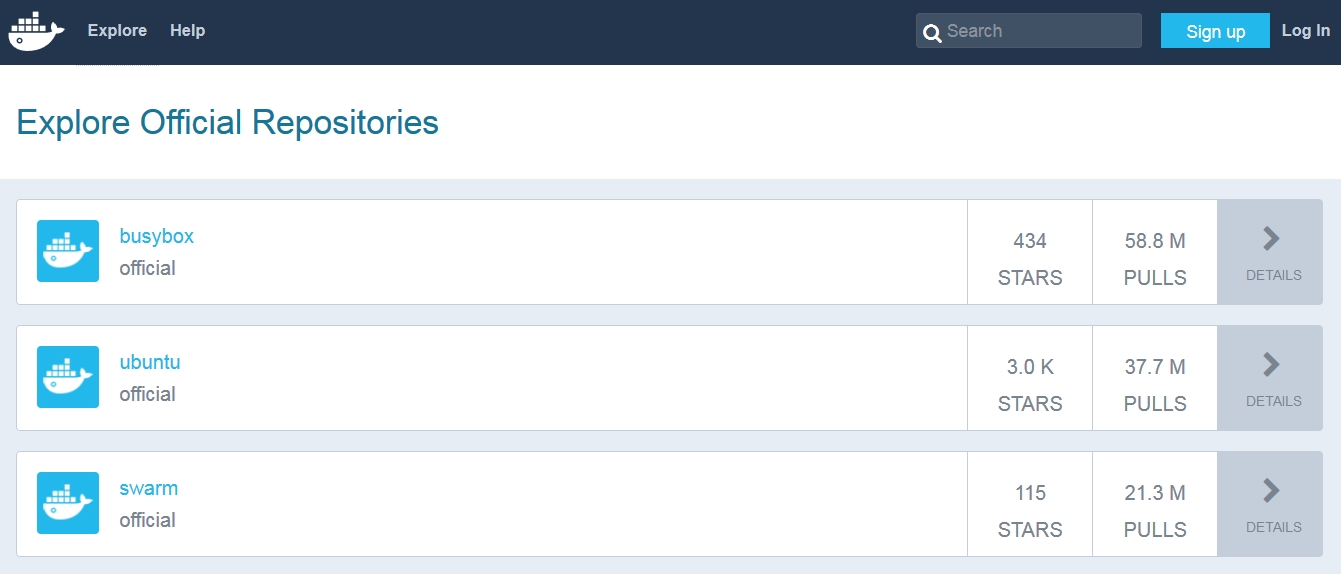
\includegraphics[width=1.0\textwidth]{./images/intro_registry.jpg}
          \caption{Web-UI des Docker Hubs mit den beliebtesten Repositories \cite{dockerHub}.}
          \label{fig:intro_registry}
      \end{figure}

      Ein Repository besteht aus mindestens einem Image. Um Images in einem Repository voneinander zu unterscheiden, werden Images Tags zugewiesen, um beispielweise mehrere Versionen eines Images in einem Repository zu kennzeichnen. Die Images werden nach dem Schema \texttt{<repository>:<tag>} identifiziert. So gibt es z.B. im offiziellen Repository des Webservers \emph{Nginx} Images mit den Tags \texttt{latest}, \texttt{1}, \texttt{1.9} und \texttt{1.9.9} \cite{dockerHubNginx}. Wenn bei dem Download kein Tag angegeben ist, wie in Kapitel wird automatisch das aktuellste Image \texttt{latest} bezogen, wie es im letzten Kapitel \ref{dockerImages} praktiziert wurde.

      % es gibt eine Trusted Registry. Die noch erklären.

      % Bsp. geben für z.B. Ubuntu mit vielen Unterversionen und dem Identifier "latest".

      % Weitere beispiele aus dockerBook: Nginx web server, MySQL Datenbank

      % Es gibt offizielle Images, die von trusted parties verwaltet werden

      Docker bietet außerdem an, private Registries zu erstellen. Diese können dann, z.B. gesichert von einer unternehmenseigenen Firewall, betrieben werden. Neben der Vertraulichkeit, bieten private Registries den Vorteil, dass sich die Speicherung und Verteilung von Images an den internen Softwareentwicklungsprozess anpassen lassen. Registries selbst können als Container betrieben werden \cite{dockerRegistry}.

      Der Zugriff auf eine Registry kann über TLS und der Verwendung eines Zertifikats, sowie \emph{basic authentication} abgesichert werden.
    \subsection{Dockerfile}
      Ein Dockerfile ist eine Datei mit selbigem Namen, die ein oder mehrere Anweisungen enthält. Letztere werden konsekutiv ausgeführt und führen jeweils zu einer neuen Schicht, die später in das generierte Image einfließt. Damit stellen Dockerfiles eine Möglichkeit dar, Images automatisiert und einfach zu generieren.
      % "einfach" schreiben? Klingt populistisch

      Eine Anweisung kann z.B. sein, ein Tool zu installieren oder zu starten, eine Umgebungsvariable festlegen oder einen Port öffnen.

      % Bsp. Dockerfile (mit drin: envvar, export port, baseimage, maintainer, authoer, apt-get)


    \subsection{Docker Architektur}
      Docker selbst ist nach einem Client-Server-Modell aufgebaut: Ein Docker-Client kommuniziert mit einem Docker-Daemon, also ein Prozess der den Server abbildet \cite{dockerUnderstandingDocker}. Beide Teile können auf einer Maschine oder einzeln auf unterschiedlichen Hosts laufen. Die Kommunikation zwischen Client und Daemon geschieht über eine RESTful API. Wie \fig \ref{fig:intro_dockerArchitecture} zeigt, ist es dadurch auch möglich Befehle entfernter Clients über ein Netzwerk an den Daemon zu senden \cite{dockerSec1}.
      % in beiden Fällen wird eine RESTful API genutzt? Setzt das docker binary nur CLI-Kommandos in REST-API-Aufrufe um?
      % Docker-Binary \texttt{docker}

      \begin{figure}[h]
          \centering
          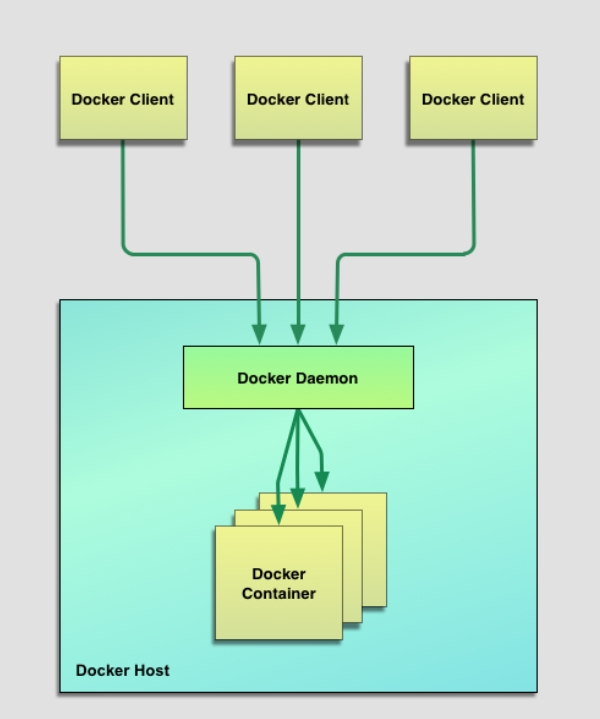
\includegraphics[width=0.9\textwidth]{./images/intro_dockerArchitecture.jpg}
          \caption{Die Client-Server-Architektur von Docker \cite{dockerUnderstandingDocker}.}
          \label{fig:intro_dockerArchitecture}
      \end{figure}

      Der Daemon kann von einer Registry Images beziehen, z.B. dem ;ffentlichen Docker Hub.
      % Kommunikation zwischen Client und Server via TCPIP oder Unix Sockets?

      Der Docker-Host selbst ist, wie in \fig \ref{fig:intro_dockerHost} dargestellt, aufgebaut. Im Idealfall läuft auf der Hardware ein minimales Linux-Betriebssystem, auf dem die Docker-Engine installiert ist. Die Engine verwaltet im Betrieb die Container, in denen in \fig \ref{fig:intro_dockerHost} die Apps A-E laufen. Wie auch in der Grafik zu sehen ist, teilen sich die Container gemeinsam verwendete Bibliotheken nach der bereits geschilderten \emph{Copy-on-write} Methode.

      \begin{figure}[h]
          \centering
          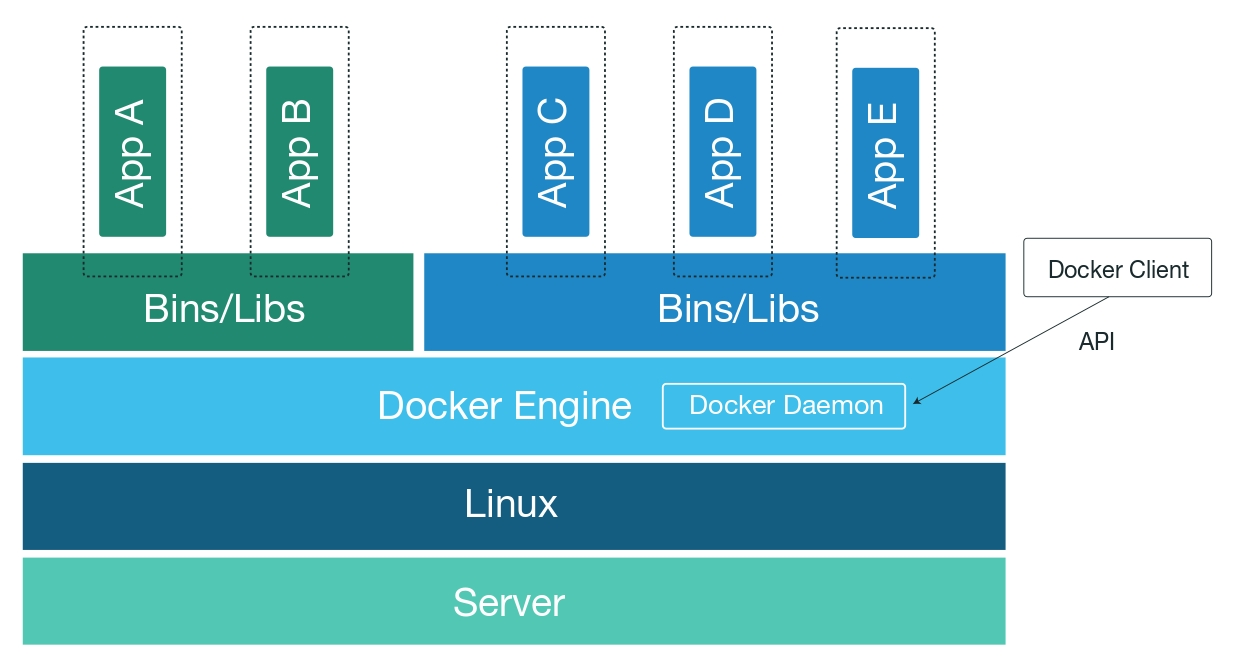
\includegraphics[width=0.9\textwidth]{./images/intro_dockerHost.jpg}
          \caption{Aufbau eines Docker-Hosts, wenn dieser unter einem Linux-Betriebssystem betrieben wird, das direkt auf der Serverhardware läuft. \cite[S.3]{dockerSecIntro}.}
          \label{fig:intro_dockerHost}
      \end{figure}

    \subsection{Containerformat \texttt{libcontainer}}
      \texttt{libcontainer} ist ein natives Linux Containerformat, das von dem Dockerteam entwickelt wurde und seit Version 0.9 das Format \emph{Linux Containers} (\emph{LXC}) ablöst \cite{dockerSec1}.

      % Seit V.XXX ist \texttt{libcontainer} das Standardformat für Docker.

\end{document}
